\documentclass[12pt,a4paper]{article}

\usepackage[english,italian]{babel}
\usepackage[utf8]{inputenc}
\usepackage{hyperref} 
\hypersetup{
    bookmarks=true,         % show bookmarks bar?
    % unicode=false,          % non-Latin characters in Acrobat’s bookmarks
    % pdftoolbar=true,        % show Acrobat’s toolbar?
    pdfmenubar=true,        % show Acrobat’s menu?
    % pdffitwindow=false,     % window fit to page when opened
    pdfstartview={FitH},    % fits the width of the page to the window
    pdftitle={Note di Algoritmi},    % title
    pdfauthor={Timoty Granziero},     % author
    % pdfsubject={},   % subject of the document 
    % pdfcreator={Creator},   % creator of the document
    % pdfproducer={Producer}, % producer of the document
    % pdfkeywords={keyword1, key2, key3}, % list of keywords
    % pdfnewwindow=true,      % links in new PDF window
    colorlinks=true,       % false: boxed links; true: colored links
    linkcolor=black,          % color of internal links (change box color with linkbordercolor)
    % citecolor=green,        % color of links to bibliography
    % filecolor=magenta,      % color of file links
    urlcolor=cyan           % color of external links
}

\usepackage{graphicx} %img/media

%\usepackage[toc]{glossaries}

\usepackage{enumitem} %lists
\usepackage[perpage]{footmisc} %footnote, starting at 1 every page

%\usepackage{listings} %coding environment

\usepackage{mathtools} %math package
\usepackage{amssymb} % N, R ... symbols

%floor and ceil
\DeclarePairedDelimiter\ceil{\lceil}{\rceil}
\DeclarePairedDelimiter\floor{\lfloor}{\rfloor}

%abs and norm
\DeclarePairedDelimiter\abs{\lvert}{\rvert}%
\DeclarePairedDelimiter\norm{\lVert}{\rVert}%

% Swap the definition of \abs* and \norm*, so that \abs
% and \norm resizes the size of the brackets, and the 
% starred version does not.
\makeatletter
\let\oldabs\abs
\def\abs{\@ifstar{\oldabs}{\oldabs*}}
%
\let\oldnorm\norm
\def\norm{\@ifstar{\oldnorm}{\oldnorm*}}
\makeatother

\usepackage{fancyhdr} %header e footer

\usepackage{clrscode3e} %algorithms pseudocode
\RequirePackage{graphics} % needed for \scalebox command

\newcommand{\authorName}{Timoty Granziero}

%liste
\renewcommand{\labelitemi}{$\circ$}
\renewcommand{\labelitemii}{$\cdot$}
\renewcommand{\labelitemiii}{$\diamond$}
\renewcommand{\labelitemiv}{$\ast$}

\author{\authorName}
\date{\today}
\title{Appunti di Algoritmi}

%header/footer setup
\fancyhf{}
\fancyhead[R]{\small\scshape\nouppercase{\leftmark}}
\fancyhead[LO]{\small\scshape\nouppercase{\rightmark}}
\fancyhead[L,RO]{\small\thepage}
\lhead{\rightmark}
\rhead{\nouppercase{\leftmark}}
\cfoot{\thepage}
%\lfoot{\authorName}

\pagestyle{fancy}

%\input{glossary.tex}
%\makeglossaries

\begin{document}

\begin{titlepage}
	\centering
	\includegraphics[width=0.50\textwidth]{img/logo_unipd_color.png}\par\vspace{1cm} %logo
	
	{\LARGE\bfseries Appunti di Algoritmi e Strutture Dati \par}
	\vspace{1cm}
	
	{\Large\bfseries a.a. 2017/2018 \par}
	
	\vspace{1cm} 

	Autore: \par
	{\bfseries \authorName \par}
	
	\vspace{1cm}

	Repository: \par
	\url{https://github.com/Vashy/ASD-Notes}
    
    \vfill
	
	% Bottom of the page
	{\large \today\par}
	
\end{titlepage}

\newpage
\tableofcontents

\frenchspacing

\newpage

\section{Lezione del 28/02/2018}

\subsection{Problem Solving}
\begin{enumerate}
	\item Formalizzazione del problema;
	\item Sviluppo dell'\textbf{algoritmo} (focus del corso);
	\item Implementazione in un programma (codice).
\end{enumerate}

\paragraph{Algoritmo} Sequenza di passi elementari che risolve il problema.\par

\begin{center}
	Input $\rightarrow$ \textbf{Algoritmo} $\rightarrow$ Output
\end{center}

\begin{quote} 
	\textit{Dato un problema, ci sono tanti algoritmi per risolverlo.}
\end{quote}

\noindent \textbf{e.g.}\footnote{For the sake of example.} Ordinamento dei numeri di una \texttt{Rubrica}.
L'idea è quella di trovare tutte le permutazioni di ogni numero.\par

\begin{center}
	30 numeri: \textit{complessità} $30! \cong 2 \times 10^{32}$ns $\Rightarrow$ \\
	$3^{19}$ anni (con \textit{ns} = nanosecondi)
\end{center}

\paragraph{std::vector} È un esempio nel \texttt{C++} delle ragioni per cui 
si studia questa materia. Nella documentazione della \texttt{STL}, 
sono riportati i seguenti:

\begin{itemize}
	\item \texttt{Random access}: complessità O(1);
	\item \texttt{Insert}: complessità O(1) ammortizzato.
\end{itemize}

Il \texttt{random access} è l'accesso a un elemento casuale del \texttt{vector}. 
O(1) implica che l'accesso avviene in tempo costante (pari a 1). \par
Per \texttt{insert} si intende l'inserimento di un nuovo elemento in coda. 
Avviene in tempo O(1) ammortizzato: questo perchè ogni N inserimenti, è 
necessario un resize del vector e una copia di tutti gli elementi nel nuovo vettore
(questa procedura è nascosta al programmatore).

\subsection{Cosa analizzeremo nel corso}

\begin{itemize}
	\item[$\bullet$] Tempo di esecuzione;
	\item[$\bullet$] Spazio (memoria);
	\medskip
	\item Correttezza;
	\item Manutenibilità.
\end{itemize}

\subsubsection{Approfondimento sul tempo di esecuzione T(n)}

\begin{itemize}
	\item \textit{P Problems}: complessità polinomiale. L'algoritmo è trattabile
	\item \textit{NP Complete}: problemi NP completi. \textbf{e.g}: Applicazione sugli algoritmi di sicurezzza. Si basano sull'assunzione che per essere risolti debbano essere considerate tutte le soluzioni possibili.
	\item \textit{NP Problems}: problemi con complessità  (ad esempio) esponenziale/fattoriale. Assolutamente non trattabili.
\end{itemize}

\begin{figure}[htb]
	\centering
	\includegraphics[height=6cm]{img/algorithm_complexity.png}
	\caption{Complessità T(n).}	
\end{figure}
	
\subsection{Problema dell'ordinamento (sorting)}
\texttt{Input}: sequenza di numeri 
\begin{center}
	$a_0 a_1 \dots a_n$;\par
\end{center}
\texttt{Output}: permutazione
\begin{center}
	$a'_0 a'_1 \dots a'_n$
\end{center}
tale che 
\begin{center}
	$a'_0 \leq a'_1 \leq \dots \leq a'_n$
\end{center}

\noindent Vedremo due algoritmi:
\begin{itemize}[noitemsep]
	\item \texttt{Insertion Sort};
	\item \texttt{Merge Sort}.
\end{itemize}

\subsection{Insertion Sort}
\href{https://en.wikipedia.org/wiki/Insertion_sort}{Insertion Sort} un algoritmo di \emph{sorting incrementale}. Viene applicato naturalmente ad esempio quando si vogliono ordinare le carte nella propria mano in una partita a scala 40: si prende ogni carta a partire da sinistra, e la si posiziona in ordine crescente.\par
\paragraph{Astrazione} Prendiamo ad esempio il seguente array:

\begin{center}
	\begin{tabular}{|l|l|l|l|l|}
		\hline
		5 & 2 & 8 & 4 & 7 \\
		\hline
	\end{tabular}
\end{center}

\noindent Partiamo dal primo elemento: 5. È già ordinato con se stesso, quindi procediamo con il secondo elemento.\par
\noindent Confronto il numero 2 con l'elemento alla sua sinistra: \par
$2 \geq 5$?  No, quindi lo inverto con l'elemento alla sua sinistra, come segue

\begin{center}
	\begin{tabular}{|l|l|l|l|l|}
		\hline
		2 & 5 & 8 & 4 & 7 \\
		\hline
	\end{tabular}
	\hspace{1cm} Key: 
	\begin{tabular}{|l|}
		\hline
		8 \\
		\hline
	\end{tabular}
\end{center}

\noindent La key analizzata è 8. \par
$8 \geq 5$? Sì, quindi è ordinato in modo corretto.

\begin{center}
	\begin{tabular}{|l|l|l|l|l|}
		\hline
		2 & 5 & 8 & 4 & 7 \\
		\hline
	\end{tabular}
	\hspace{1cm} Key: 
	\begin{tabular}{|l|}
		\hline
		4 \\
		\hline
	\end{tabular}
\end{center}

\noindent La key analizzata è 4.\par
$4 \geq 8$? No, quindi lo sposto a sinistra invertendolo con 8.\par 
$4 \geq 5$? No, lo sposto a sinistra invertendolo con 5.\par
$4 \geq 2$? Sì, quindi è nella posizione corretta.

\begin{center}
	\begin{tabular}{|l|l|l|l|l|}
		\hline
		2 & 4 & 5 & 8 & 7 \\
		\hline
	\end{tabular}
	\hspace{1cm} Key: 
	\begin{tabular}{|l|}
		\hline
		7 \\
		\hline
	\end{tabular}
\end{center}

\noindent Key analizzata 7. \par
$7 \geq 8$? No, lo sposto a sinistra invertendolo con 8.\par
$7 \geq 5$? Sì, è nella posizione corretta.\par

\smallskip
\noindent Ottengo l'array ordinato:

\begin{center}
	\begin{tabular}{|l|l|l|l|l|}
		\hline
		2 & 4 & 5 & 7 & 8 \\
		\hline
	\end{tabular}
\end{center}

\newpage

\paragraph{Algorimo} Passiamo ora all'implementazione dell'algoritmo, con uno pseudocodice similare a \texttt{Python}\footnote{\textbf{ATTENZIONE}: verranno usati array con indici
che partono da 1.}\par

\bigskip

\texttt{Input}: $A[1, \twodots ,n]$, $A.length$.

\begin{center}
	È noto che: 
	$A[i] \leq key < A[i+1]$
\end{center}

\paragraph{Pseudocodice} Segue lo pseudocodice dell'\texttt{Insertion Sort}.

\begin{codebox}
\Procname{$\proc{Insertion-Sort}(A)$}
\li $n \gets \attrib{A}{length}$
\li \For $j \gets 2$ \To $n$
	\Comment il primo elemento è già ordinato
\li		\Do
			$\id{key} \gets A[j]$ 
			\Comment $A[1 \twodots j-1]$ ordinato
\li			$i \gets j-1$
\li			\While $i > 0$ and $A[i] > \id{key}$
\li				\Do
					$A[i+1] \gets A[i]$
\li					$i \gets i-1$
				\End
\li			$A[i+1] \gets \id{key}$
		\End
\end{codebox}

\vspace{0.5cm}

Quando il \texttt{while} termina, ci sono due casi: 
\begin{itemize}
	\item[$\circ$] \texttt{i = 0}: tutti gli elementi prima di \texttt{j} 
	sono maggiori di \texttt{key}; \texttt{key} va al primo posto (1);
	\item[$\circ$] \texttt{(i > 0) and (A[i] $\leq$ key)}: \texttt{A[i+1] = key}.
\end{itemize}

\subsubsection{Invarianti e correttezza}

\paragraph{for} \texttt{A[1$\twodots$j-1]} è ordinato e contiene gli 
elementi in \texttt{(1,j-1)} iniziali.

\paragraph{while} \texttt{A[1$\twodots$i]A[i+2$\twodots$j]} ordinato e 
\texttt{A[i+2$\twodots$j] > key}. \par
\vspace{0.5cm}
In uscita abbiamo: 
\begin{itemize}[noitemsep]
	\item[$\circ$] \texttt{j = n+1}; \par
	\item[$\circ$] \texttt{A[1$\twodots$n]} ordinato, come da invariante: 
	vale \texttt{A[1$\twodots$j-1]}	ordinato, e \texttt{j} vale \texttt{n+1}.
\end{itemize} \newpage
\section{Lezione del 02/03/2018}

\subsection{Modello dei costi}
\paragraph{Assunzione} Tutte le istruzioni richiedono un tempo \underline{costante}.

Rivediamo l'algoritmo:

\begin{codebox}
\Procname{$\proc{Insertion-Sort}(A)$}
\li $n \gets \attrib{A}{length}$
\li \For $j \gets 2$ \To $n$
	\Comment il primo elemento è già ordinato
\li		\Do
			$\id{key} \gets A[j]$ 
			\Comment $A[1 \twodots j-1]$ ordinato
\li			$i \gets j-1$
\li			\While $i > 0$ and $A[i] > \id{key}$
\li				\Do
					$A[i+1] \gets A[i]$
\li					$i \gets i-1$
				\End
\li			$A[i+1] \gets \id{key}$
		\End
\end{codebox}

Diamo il nome $c_0$ alla chiamata del metodo, \texttt{InsertionSort(A)};
A ogni riga numerata, diamo il nome $c_1, c_2,\twodots ,c_8$
\footnote{($c_1$ corrisponde alla riga 1, $c_2$ alla riga 2 e così via).}.\par
Vediamo il \emph{costo} di ogni istruzione:

\begin{itemize}
    \item[] $\boldsymbol{c_0} \rightarrow 1$
    \item[] $\boldsymbol{c_1} \rightarrow 1$
    \item[] $\boldsymbol{c_2} \rightarrow n$
    \item[] $\boldsymbol{c_3} \rightarrow (n-1)$
    \item[] $\boldsymbol{c_4} \rightarrow (n-1)$
    \item[] $\boldsymbol{c_5} \rightarrow \displaystyle\sum_{j=2}^{n} t_j+1$
    \item[] $\boldsymbol{c_6}, \boldsymbol{c_7} \rightarrow \displaystyle\sum_{j=2}^{n} t_j$
    \item[] $\boldsymbol{c_8} \rightarrow (n-1)$
\end{itemize}

\subsection{Complessità di IS} \label{is:complessita}
\begin{displaymath}
    T^{IS}(n) = c_0 + c_1 + c_2n + (c_3+c_4+c_8)(n-1)
    + c_5\displaystyle\sum_{j=2}^{n}(t_j+1) + (c_6+c_7)\displaystyle\sum_{j=2}^{n}t_j
\end{displaymath}

$\boldsymbol{t_j}$ dipende, oltre che da $n$, dall'istanza dell'array
che stiamo considerando.
È chiaro che questo calcolo non da indicazioni precise sull'effettiva
complessità dell'algoritmo.\par

\bigskip
Andiamo ad analizzare i 3 possibili casi:

\begin{enumerate}[label=\emph{\alph*})]
    \item Caso migliore (\ref{is:casomigliore})
    \item Caso peggiore (\ref{is:casopeggiore})
    \item Caso medio (\ref{is:casomedio})
\end{enumerate}

\subsubsection{Caso migliore} \label{is:casomigliore}

$\rightarrow A$ ordinato $\Rightarrow t_j = 0 $ $\forall j$

\bigskip
La \textbf{complessità} diventa:
\begin{displaymath}
    T^{IS}_{min}(n) = c_0 + c_1 + c_2n + (c_3+c_4+c_5+c_8)(n-1) 
    = an+b \approx n
\end{displaymath}

Ossia, si comporta come $n$. Il \emph{caso migliore} \textbf{non}
è interessante, visto che è improbabile si presenti.

\subsubsection{Caso peggiore} \label{is:casopeggiore}

$\rightarrow A$ ordinato in senso inverso $\Rightarrow \forall j$ $t_j = j-1$ \par
\bigskip
La \textbf{complessità} diventa: 

\begin{displaymath}
    T^{IS}_{max}(n) = c_0 + c_1 + c_2n + (c_3+c_4+c_8)(n-1)
    + c_5\displaystyle\sum_{j=2}^{n}j + (c_6+c_7)
    \displaystyle\sum_{j=2}^{n}(j-1)
\end{displaymath}

Per valutare il costo di $\displaystyle\sum_{j=2}^{n}j$ e di 
$\displaystyle\sum_{j=2}^{n}(j-1)$, usiamo la \textbf{somma di Gauss}: \par

\begin{equation}
    \displaystyle\sum_{i=1}^{n}i = \frac{n(n+1)}{2}
\end{equation}
\newpage
Otteniamo:

\begin{displaymath}
    \displaystyle\sum_{j=2}^{n}j = \frac{n(n+1)}{2}-1
\end{displaymath}

\begin{displaymath}
    \displaystyle\sum_{j=2}^{n}(j-1) = \displaystyle\sum_{i=1}^{n}n = \frac{(n-1)n}{2}
\end{displaymath}

Per finire, ricalcoliamo $T^{IS}_{max}(n)$

\begin{displaymath}
    T^{IS}_{max}(n) = a'n^2+b'n+c' \approx n^2
\end{displaymath}

\subsubsection{Caso medio} \label{is:casomedio}
Il caso medio è \emph{difficile da calcolare}, e in una considerevole parte dei casi,
coincide con il caso peggiore.\par
Comunque, l'idea è la seguente:

\begin{align*}
    \frac{\displaystyle\sum_{\text{perm. di input}}T^{IS}(p)}{n!} \approx n^2 && 
        \text{posso pensare che } t_j \cong \frac{j-1}{2}
\end{align*}

\subsection{Divide et Impera}

Un algoritmo di sorting \emph{divide et impera} si può suddividere in 3 fasi:

\begin{description}
    \item[divide] divide il problema dato in sottoproblemi più piccoli;
    \item[impera] risolve i sottoproblemi:
    \begin{itemize}
        \item ricorsivamente;
        \item la soluzione è nota (e.g. array con un elemento);
    \end{itemize}
    \item[combina] compone le soluzioni dei sottoproblemi in una soluzione del 
        problema originale.
\end{description}

\subsection{Merge Sort}
\href{https://en.wikipedia.org/wiki/Merge_sort}{Merge Sort}\footnote{Si %
consiglia di dare uno sguardo all'algoritmo anche da altre fonti, poichè presentarlo %
graficamente in \LaTeX, come è stato visto a lezione, non è facile.} è un 
esempio di algoritmo \emph{divide et impera}. Andiamo ad analizzarlo.

\paragraph{Astrazione} Consideriamo il seguente array A.
\begin{center}
	\begin{tabular}{|l|l|l|l||l|l|l|l|}
		\hline
		5 & 2 & 4 & 7 & 1 & 2 & 3 & 6 \\
		\hline
	\end{tabular}
\end{center}

Lo divido a metà, ottenendo due parti separate.

\begin{center}
	\begin{tabular}{|l|l|l|l|}
		\hline
		5 & 2 & 4 & 7 \\
		\hline
	\end{tabular}
	\hspace{1cm}
	\begin{tabular}{|l|l|l|l|}
		\hline
		1 & 2 & 3 & 6 \\
		\hline
	\end{tabular}
\end{center}

Consideriamo il primo, ossia \texttt{A[1$\twodots$4]} (A originale). Divido anche questo a metà.

\begin{center}
	\begin{tabular}{|l|l|}
		\hline
		5 & 2 \\
		\hline
	\end{tabular}
	\hspace{1cm}
	\begin{tabular}{|l|l|}
		\hline
		4 & 7 \\
		\hline
	\end{tabular}
\end{center}

Divido nuovamente a metà, ottenendo:

\begin{center}
	\begin{tabular}{|l|}
		\hline
		5 \\
		\hline
	\end{tabular}
	\hspace{1cm}
	\begin{tabular}{|l|}
		\hline
		2 \\
		\hline
	\end{tabular}
\end{center}

5 e 2 sono due blocchi già ordinati. Scelgo il minore tra i due e lo metto in prima 
posizione, mentre l'altro in seconda posizione, ottenendo un blocco composto da 2 e 5.\par
Riprendo con il blocco composto da 4 e 7. Lo divido in due blocchi da un elemento. Faccio lo stesso procedimento 
fatto per 2 e 5: metto in prima posizione 4 e in seconda posizione 7. La situazione
è la seguente:

\begin{center}
	\begin{tabular}{|l|l|}
		\hline
		2 & 5 \\
		\hline
	\end{tabular}
	\hspace{1cm}
	\begin{tabular}{|l|l|}
		\hline
		4 & 7 \\
		\hline
	\end{tabular}
\end{center}

So che i blocchi ottenuti contengono elementi ordinati. Con questa assunzione, posso ragionare 
nel seguente modo: considero il primo elemento dei due blocchi (2 e 4 in questo caso) e metto 
in prima posizione il minore tra i due. Ora considero il successivo elemento del blocco che è stato scelto e lo stesso elemento dell'altro blocco, e inserisco nell'array l'elemento minore. Continuo fino ad 
ottenere un blocco ordinato.

\begin{center}
	\begin{tabular}{|l|l|l|l|}
		\hline
		2 & 4 & 5 & 7 \\
		\hline
	\end{tabular}
\end{center}

Faccio lo stesso procedimento con la parte di array originale \texttt{A[5$\twodots$8]}, ottenendo

\begin{center}
	\begin{tabular}{|l|l|l|l|}
		\hline
		2 & 4 & 5 & 7 \\
		\hline
	\end{tabular}
	\hspace{1cm}
	\begin{tabular}{|l|l|l|l|}
		\hline
		1 & 2 & 3 & 6 \\
		\hline
	\end{tabular}
\end{center}

A questo punto, i blocchi da 4 contengono elementi tra loro ordinati. Faccio lo stesso ragionamento
usato per comporli, per ottenere l'array originale ordinato. Considero\footnote{Questo procedimento è stato applicato %
anche ai passaggi precedenti; qui è spiegato più rigorosamente.}:
\begin{itemize}[noitemsep]
    \item \texttt{L[1$\twodots$4] $=$ A[1$\twodots$4]}: indice $i = 1$ per scorrerlo;
    \item \texttt{R[1$\twodots$4] $=$ A[5$\twodots$8]}: indice $j = 1$ per scorrerlo;
\end{itemize}

Valuto \texttt{L[i]} e \texttt{R[j]}. \par
\begin{itemize}[noitemsep]
    \item Se \texttt{L[i]} $\leq$ \texttt{R[j]}, inserisco \texttt{L[i]} e incremento \texttt{i}. \par
    \item Altrimenti, inserisco \texttt{R[j]} e incremento \texttt{j}.
    \item Itero finchè entrambi gli indici non sono out of bounds.
\end{itemize}

\paragraph{Pseudocodice} Segue lo pseudocodice del 
\texttt{Merge Sort}.

\begin{codebox}
\Procname{$\proc{Merge-Sort}(A,p,r)$}
\li \If $p < r$
\li     \Then
            $q \gets (p + r) / 2$ 
        \Comment arrotondato per difetto
\li         $\proc{Merge-Sort}(A,p,q)$
        \Comment ordina \texttt{A[p$\twodots$q]}
\li         $\proc{Merge-Sort}(A,q+1,r)$
        \Comment ordina \texttt{A[q+1$\twodots$r]}
\li         $\proc{Merge}(A,p,q,r)$
        \Comment ``Merge'' dei due sotto-array 
        \End
\end{codebox}

\begin{codebox}
\Procname{$\proc{Merge}(A,p,q,r)$}
\li $\id{n1} \gets q-p+1$
    \Comment gli indici partono da 1
\li $\id{n2} \gets r-q$
\zi \Comment \kw{L} sotto-array sx, \kw{R} sotto-array dx
\li \For $i \gets 1$ \To $\id{n1}$
\li     \Do
            $L[i] \gets A[p+i-1]$
\li         \For $j \gets 1$ \To $\id{n2}$
\li             \Do
                    $R[j] \gets A[q+j]$
                \End
\li         $L[\id{n1}+1] \gets R[\id{n2}+1] \gets \infty$
\li         $i \gets j \gets 1$
\li         \For $k = p$ \To $r$
\li             \Do
                    \If $L[i] \leq R[j]$
\li                     \Then
                            $A[k] \gets L[i]$
\li                         $i \gets i+1$
\li                     \Else
                    \Comment \texttt{L[i]} $>$ \texttt{R[j]}
\li                            $A[k] \gets R[j]$
\li                         $j \gets j+1$
                        \End
                \End
        \End
\end{codebox}

\subsubsection{Invarianti e correttezza}

\textbf{L} e \textbf{R} contengono rispettivamente 
\texttt{A[p$\twodots$q]} e \texttt{A[q+1$\twodots$r]}. 
L'indice \texttt{k} scorre \texttt{A}. Il sotto-array \texttt{A[p$\twodots$k-1]}
è ordinato, e contiene \texttt{L[1$\twodots$i-1]} e \texttt{R[1$\twodots$j-1]}.

\begin{center}
    $A[p \twodots k-1] \leq L[i \twodots n1], R[j \twodots n2]$ \\
    $\Downarrow$ \\
    $A[p \twodots k-1] = A[p \twodots r+1-1] \implies A[p \twodots r] \text{ ordinato}$
\end{center}

\paragraph{Dimostrazione per induzione su r-p} 
\begin{itemize}
    \item[$\Rightarrow$] Se $r-p == 0 $ (oppure $-1$) abbiamo al
    più un elemento $\implies$ array già ordinato.
    \item[$\Rightarrow$] Se $r-p > 0$, vale 
    $\#\text{elem}(A[p \twodots q]),\#\text{elem}(A[q+1 \twodots r]) 
    < \#\text{elem}(A[p \twodots r])$.
    Per ipotesi induttiva:
    \begin{itemize}
        \item \texttt{Merge-sort(A,p,q)} ordina \texttt{A[p$\twodots$q]};
        \item \texttt{Merge-sort(A,q+1,r)} ordina \texttt{A[q+1$\twodots$r]}; \par
        Per correttezza di \texttt{Merge()}, dopo la sua chiamata ottengo 
        \texttt{A[p$\twodots$r]} ordinato.
    \end{itemize}
\end{itemize}  
\section{Lezione del 07/03/2018}

\subsection{Approfondimento sull'induzione}

\subsubsection{Induzione ordinaria} 

Proprietà $P(n)$, e.g., $ = $ ``Se $n$ è pari, $n+1$ è dispari'' oppure 
``tutti i grafi con $n$ nodi \dots ''.\par
Per dimostrare che $P(n)$ vale per ogni $n$
\begin{itemize}
	\item $P(0)$: \textbf{caso base};
	\item assumo vera $P(n) \rightarrow $ dimostro $P(n+1)$, allora $P(n)$
	è vera per ogni $n$.
\end{itemize}

\subsubsection{Induzione completa}
\begin{itemize}
	\item $\big[ P(0) \big]$ (non necessaria, è un'istanza del passo successivo);
	\item dimostro $P(m) \ \forall m<n \rightarrow $ vale $P(n) \ \forall n$.  
\end{itemize}

\subsection{Complessità di Merge Sort}

$n = \#$elementi da ordinare\footnote{Il simbolo \# verrà usato per indicare la cardinalità di un insieme.}

\paragraph{Merge(A,p,q,r)}
\begin{itemize}
	\item[] \textbf{inizializzazione}: $a'n+b'$;
	\item[] \textbf{ciclo}: $a'n+b'$;
\end{itemize}

Sommandoli, ottengo una complessità all'incirca di:
\begin{displaymath}
	T^{merge}(n) = an+b
\end{displaymath}

Nel dettaglio: 

\[ T^{MS}(n) =
\begin{cases}
	c_0       & \quad \text{se } n \leq 1 \\
	T^{MS}(n_1)+T^{MS}(n_2)+T^{merge}(n)  & \quad \text{altrimenti}
\end{cases}
\]

\begin{center}
	$\Downarrow$ \\
\end{center}

\[ T^{MS}(n) =
\begin{cases}
c_0       & \quad \text{se } n \leq 1 \\
T^{MS}(n_1)+T^{MS}(n_2)+an+b  & \quad \text{altrimenti}
\end{cases}
\]

con 

\begin{itemize}
	\item[] $T^{MS}(n_1) = \floor{\frac{n}{2}}$
	\item[] $T^{MS}(n_2) = \ceil{\frac{n}{2}}$
\end{itemize}

%\subsubsection{Complessità }

\begin{align*}
	T^{MS}(n) \\
	an+b
\end{align*}
\begin{align*}
	T^{MS}(n_1) && T^{MS}(n_2) \\
	an_1+b && an_2+b
\end{align*}
\begin{align*}
T^{MS}(n_{11}) && T^{MS}(n_{12}) && T^{MS}(n_{21}) && T^{MS}(n_{22}) \\
an_{11}+b && an_{12}+b && an_{21}+b && an_{22}+b
\end{align*}
\begin{center}
	\dots
\end{center}
\begin{align*}
	c_0 && c_0 && \dots && \dots && \dots && c_0 && c_0 \\
\end{align*}

Otteniamo $c_0$ ripetuto $n$ volte all'ultimo livello dell'albero. Vediamo nel dettaglio la complessità
nelle varie iterazioni.
\begin{itemize}
	\item[] $\boldsymbol{i=0}$ \hspace{0.5cm} $an+b$
	\item[] $\boldsymbol{i=1}$ \hspace{0.5cm} $a(n_1+n_2)+2b \approx an+2b$
	\item[] $\boldsymbol{i=2}$ \hspace{0.5cm} $a(n_{11}+n_{12}+n_{21}+n_{22})+4b \approx an+4b$
	\item[] \dots
	\item[] $\boldsymbol{i=h}$ \hspace{0.5cm} $c_0n$
\end{itemize}

Poniamo $n=2^h$. Abbiamo

\begin{align*}
	T^{MS}(n) 	& = \displaystyle\sum_{i=0}^{h-1}(an+2^ib)+c_0n \\
				& = anh+b\displaystyle\sum_{i=0}^{h-1}2^i && \text{($h= \log_2n$)}\\
				& = an \log_2n + b2^h - b + c_0n && \text{($2^h=n$)} \\
				& = an \log_2n + (b+c_0)n - b
\end{align*}
\begin{displaymath}
	T^{MS}(n) = an \log_2n + b''n + c'' \approx n \log_2n
\end{displaymath}

\subsection{Confronto tra IS e MS}

\begin{gather*}
	T^{IS}(n) = a'n^2 + b'n + c' \\
	T^{MS}(n) = an \log_2n + b''n + c''
\end{gather*}

Posso calcolare il limite del rapporto:
\begin{displaymath}
	\lim_{n \to +\infty} \frac{T^{MS}(n)}{T^{IS}(n)} = \lim_{n \to +\infty} \frac{an \log_2n + b''n + c''}{a'n^2 + b'n + c'} = 0
\end{displaymath}

Per definizione
\begin{gather*}
	\forall \varepsilon > 0 \ \exists n_0 : \forall n \geq n_0 \quad \frac{T^{MS}(n)}{T^{IS}(n)} < \varepsilon \\
	\Downarrow
\end{gather*}
\begin{align*}
	T^{MS}(n) < \varepsilon T^{IS}(n) = \frac{T^{IS}}{m} && \text{(Ponendo, ad esempio, $\varepsilon = \frac{1}{m}$)}
\end{align*}

Detto a parole, c'è un certo $n$ oltre il quale, ad esempio, \texttt{Merge Sort} su un \emph{Commodore 64} 
esegue più velocemente di un \texttt{Insertion Sort} su una macchina moderna, come mostrato nella seguente 
tabella.
\begin{center}
	\begin{tabular}{l|c|c}
		$n$ & $T^{IS}(n)=n^2$ & $T^{MS}(n)=n \log n$ \\
		\hline
		10 & $0.1ns$ & $0.033ns$ \\
		\hline
		1000 & $1ms$ & $10\mu s$ \\
		\hline
		$10^6$ & 17 minuti & $20ms$ \\
		\hline
		$10^9$ & 70 anni & $30s$ \\
	\end{tabular}
\end{center}
\section{Lezione dell'08/03/2018}

\subsection{Notazione asintotica}
Il \textbf{tempo di esecuzione} è difficile da calcolare, come visto nella sezione \ref{is:complessita}. 
Il modo in cui è stato calcolato è pieno di dettagli ``inutili''.\par
Rivediamo le complessità di Insertion Sort e Merge Sort:
\begin{gather*}
	T^{IS} = an^2 + bn + c \\
	T^{MS} = an \log_2 n + bn + c
\end{gather*}

A noi interessa calcolare $T(n)$ per $n$ ``grande''. Non consideriamo le costanti moltiplicative, che sono non fondamentali. Ecco una lista di possibili complessità ordinate in senso decrescente (le prime due categorie appartengono alla classe degli \emph{NP problems}, ossia non trattabili):

\begin{itemize}[noitemsep]
	\item $3^n$
	\item $2^n$
	\medskip
	\item $n^k$
	\item $n^2$
	\item $n \log n$
	\item $n$
	\item $\log n$
	\item $1$
\end{itemize}

Prendiamo in esame due funzioni: $f(n)$, $g(n)$:

\begin{displaymath}
f, g: \mathbb{R}^+ \rightarrow \mathbb{R}^+
\end{displaymath}

\begin{itemize}
	\item $f(n)$ è la funzione in esame della complessità del nostro problema P;
	\item $g(n)$ è la funzione che, moltiplicata per un'opportuna costante $c_i$, dopo un certo $n$, fa da 
	limite superiore o inferiore per ogni punto di $f(n)$.
\end{itemize}
\newpage
\subsubsection{Limite asintotico superiore}
Data $g(n)$, indichiamo con $O \big(g(n) \big)$ il \emph{limite asintotico superiore}, definito come segue:
\begin{displaymath}
	O \big(g(n) \big) = \{ f(n) \ \vert \ \exists c > 0 \quad \exists n_0 (\in \mathbb{N}) \ \vert \ \forall n \geq n_0 \Rightarrow (0 \leq) f(n) \leq c \cdot g(n) \}
\end{displaymath}

\begin{center}
	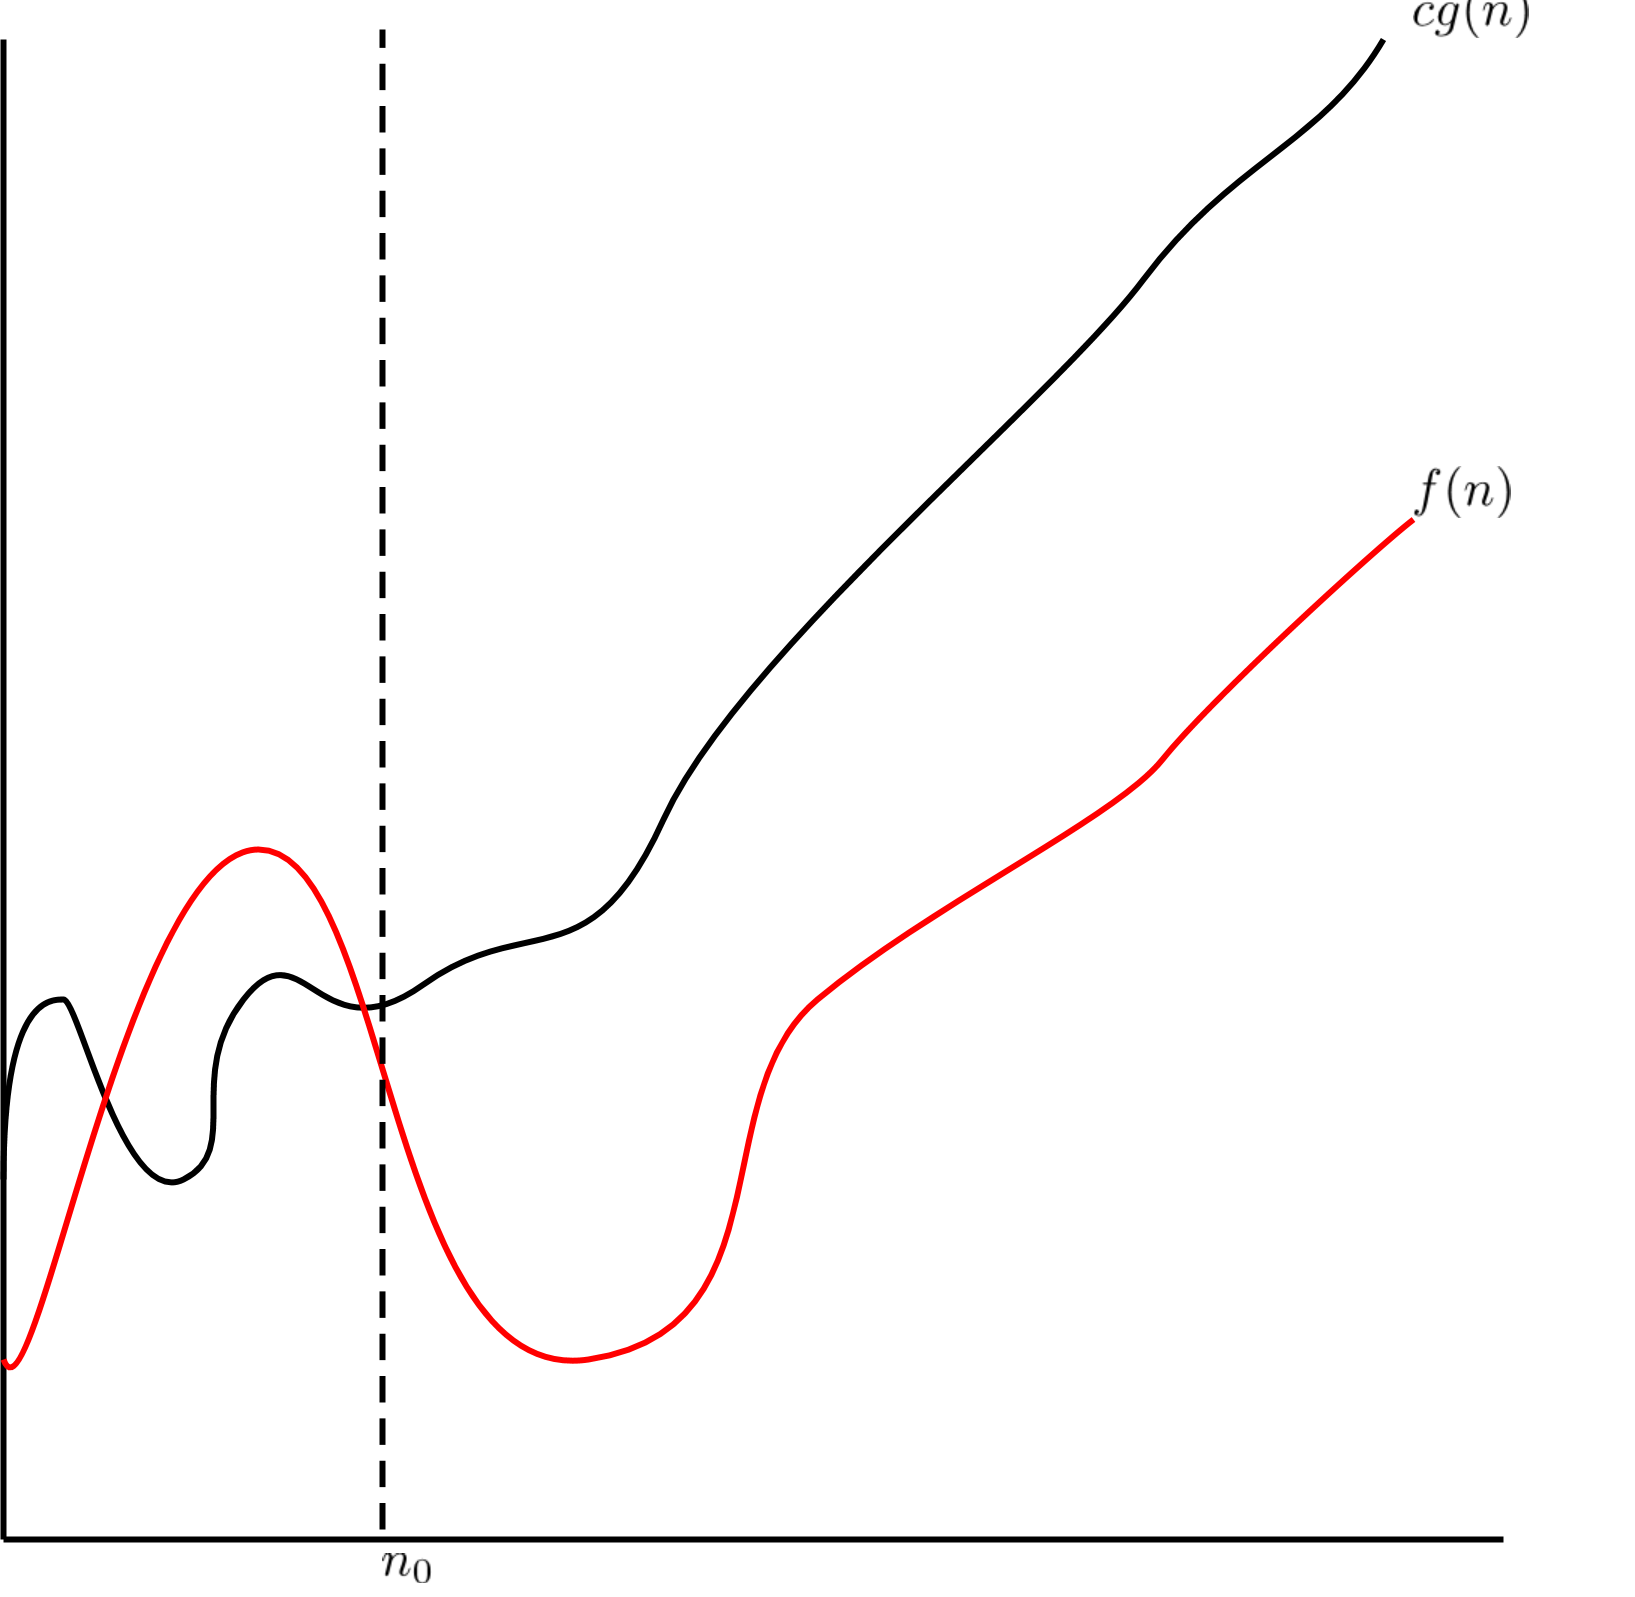
\includegraphics[width=0.80\textwidth]{img/plots/plotO.png}
\end{center}

\paragraph{Esempi}
\begin{itemize}
	\item $f_1(n) = 2n^2 + 5n + 3 = O \big(g(n^2) \big)$ ? Sì. \par
	Deve valere $f_1(n) < cn^2 \qquad \exists c > 0, \ n \geq n_0$ \par
	Ipotizziamo $c = 3$
	\begin{align*}
		2n^2 + 5n + 3 & \leq 3n^2 \\
		n^2 - 5n - 3 & \geq 0 \\
		\frac{5 \pm \sqrt{2 \cdot 5 + 12}}{2} = \frac{5 \pm \sqrt{37}}{2} \cong 5.54 && \text{(Non considero la soluzione} \\ && \text{negativa, poiché siamo in } \mathbb{R}^+ \text{)}
	\end{align*}
	\begin{center}
		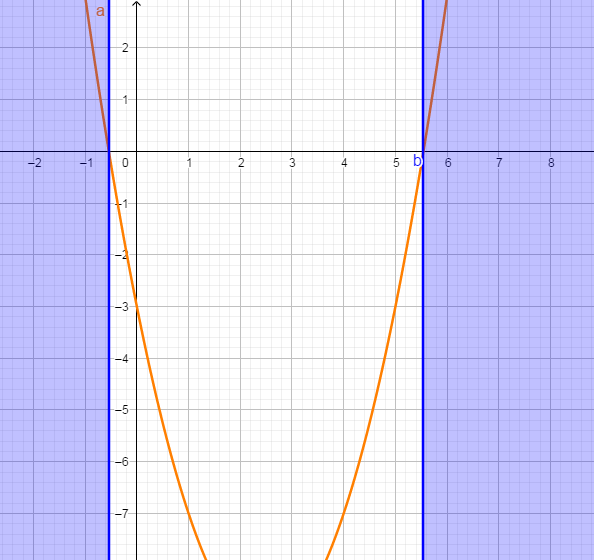
\includegraphics[height=6cm]{img/parabola-plot1.png}
	\end{center}
	
	Prendo $c = 3$ e $n_0 = 6$. Vale dunque:
	\begin{displaymath}
		f_1(n) \leq cn^2 \quad \forall n \geq n_0
	\end{displaymath}

	\item $f_1(n) = O \big(g(n^3) \big)$ ? Sì. \par
	$c = 3 $\par
	$n_0 = 6 \quad \forall n \geq n_0$ \par
	$f_1(n) \leq cn^2 \leq cn^3$
	
	\item $f_2(n) = 2 + \sin (n) = O(1)$ ? Sì. \par
	$-1 \leq \sin (n) \leq 1$ \par
	$1 \leq f_2(n) \leq 3$ \par
	Vale la seguente
	\begin{gather*}
		\exists c > 0 \quad \exists n_0 : n \geq n_0 \Rightarrow f_2(n) \leq c \cdot 1 \\
		\text{ok per } c = 3, \ n_0 = 0
	\end{gather*}
\end{itemize}
\newpage
\subsubsection{Limite asintotico inferiore}
Data $g(n)$, indichiamo con $\Omega \big(g(n) \big)$ il \emph{limite asintotico inferiore}, definito come segue:
\begin{displaymath}
	\Omega \big(g(n) \big) = \{ f(n) \ \vert \ \exists c > 0 \quad \exists n_0 (\in \mathbb{N}) \ \vert \ \forall n \geq n_0 \Rightarrow c \cdot g(n) \leq f(n) \}
\end{displaymath}

\begin{center}
	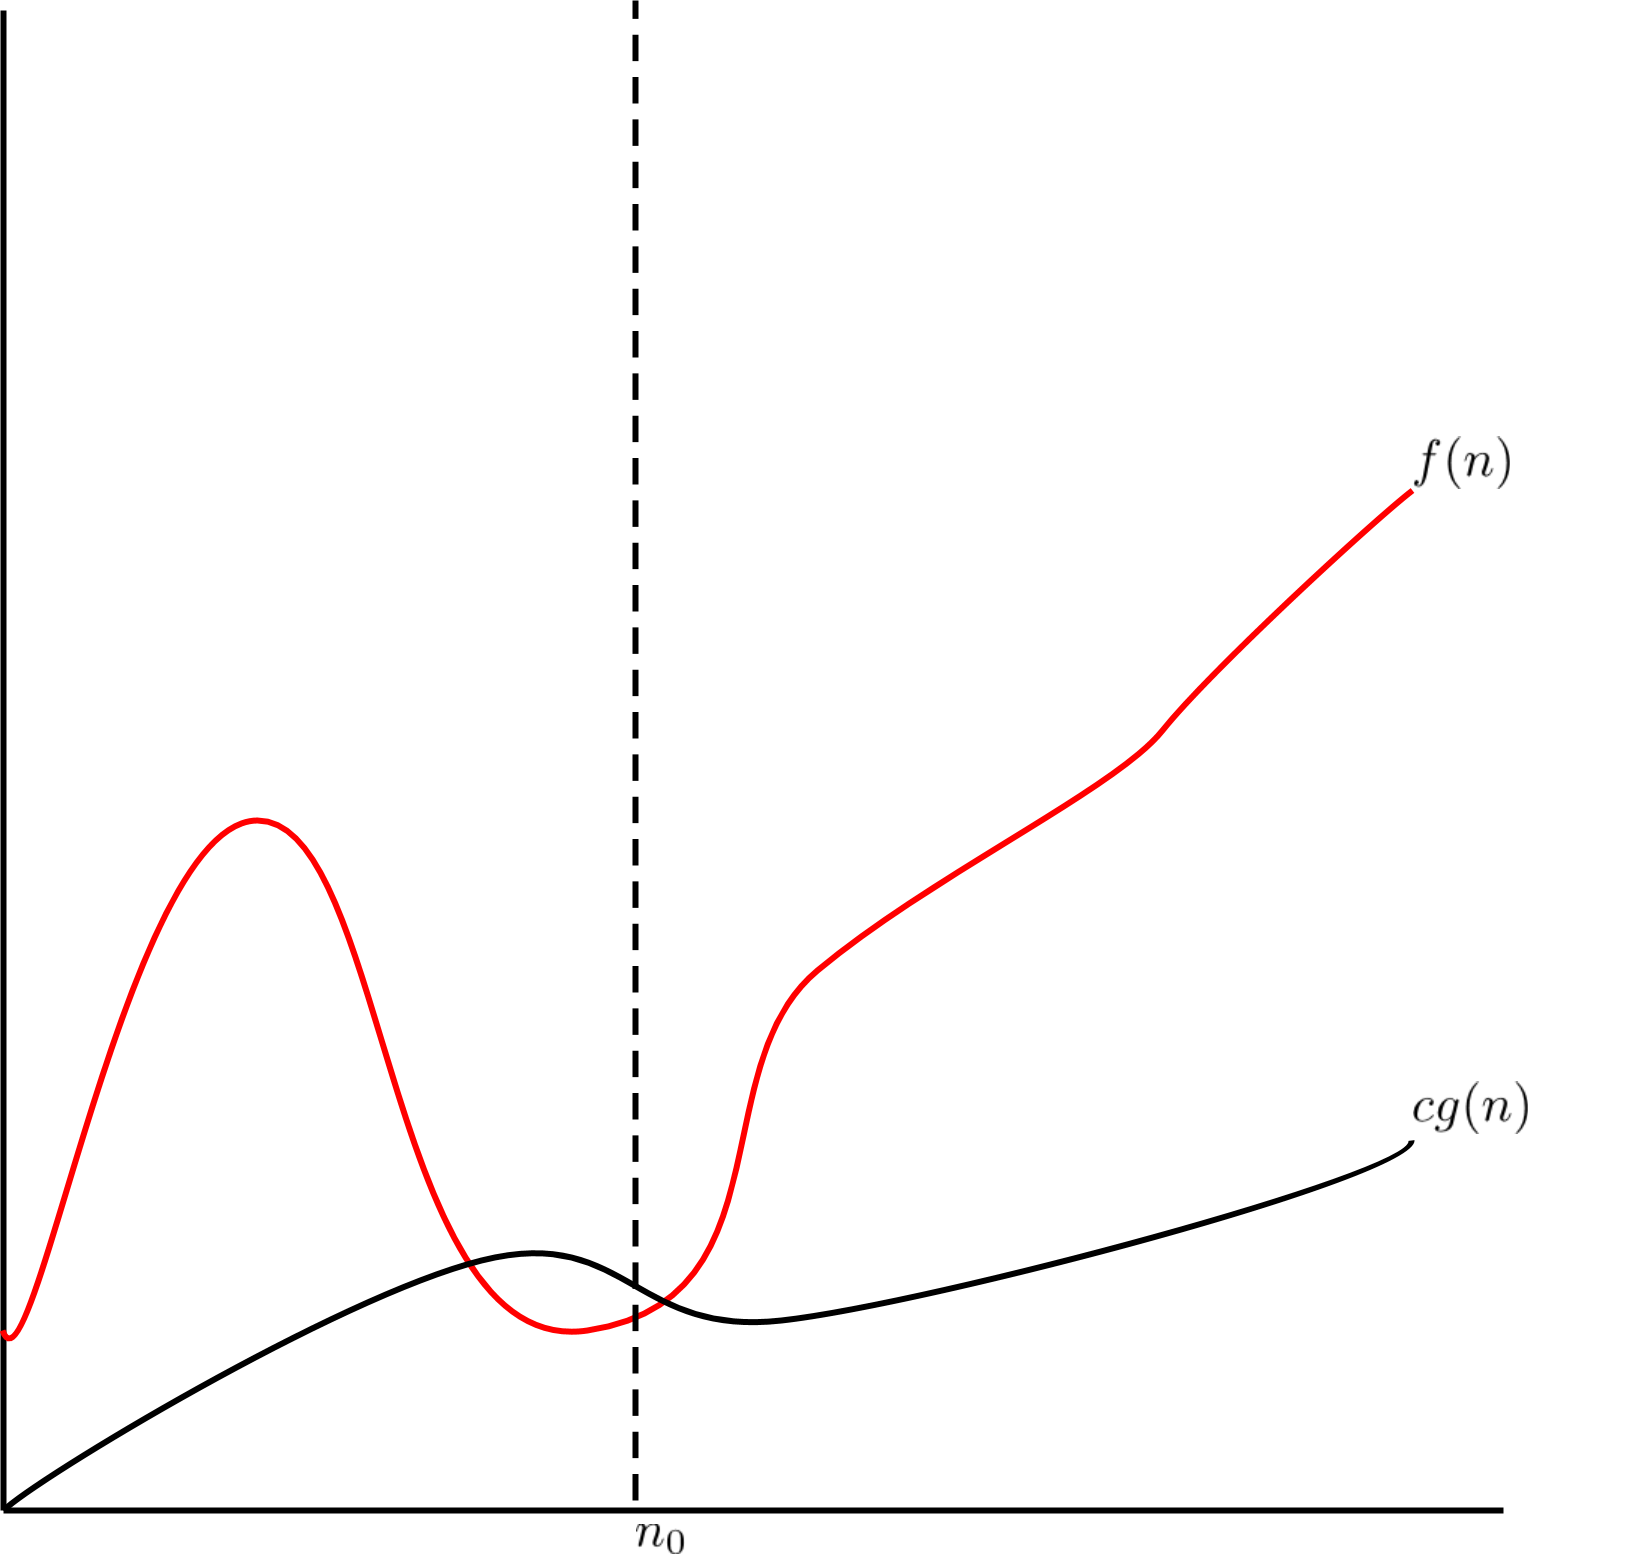
\includegraphics[width=0.80\textwidth]{img/plots/plotomega.png}
\end{center}

\paragraph{Esempi}
\begin{itemize}
	\item $f_1(n) = 2n^2 + 5n + 3 = \Omega \big(g(n^2) \big)$ ? Sì.\par
	Deve valere: \par
	\begin{displaymath}
		\exists c > 0 \quad \exists n_0 : \forall n \geq n_0 \Rightarrow cn^2 \leq 2n + 5n + 3
	\end{displaymath}
	Basta porre $c = 1$, $n_0 = 0$.
	
	\item $f_2(n) = 2 + \sin (n) = \Omega (1)$ ? Sì.
	\begin{displaymath}
		1 \leq f_2(n) \leq 3 \quad c = 1, \ n_0 = 0
	\end{displaymath}
\end{itemize}

\subsubsection{Limite asintotico stretto}
Data $g(n)$, indichiamo con $\Theta \big( g(n) \big)$ il \emph{limite asintotico stretto}, definito come segue:
\begin{multline*}
	\Theta \big( g(n) \big) = \{ f(n) \ \vert \ \exists c_1, c_2 > 0 \quad \exists n_0 (\in \mathbb{N}) \ \vert \ \forall n \geq n_0 \\ 
	\Rightarrow c_1 \cdot g(n) \leq f(n) \leq c_2 \cdot g(n) \}
\end{multline*}

\begin{center}
	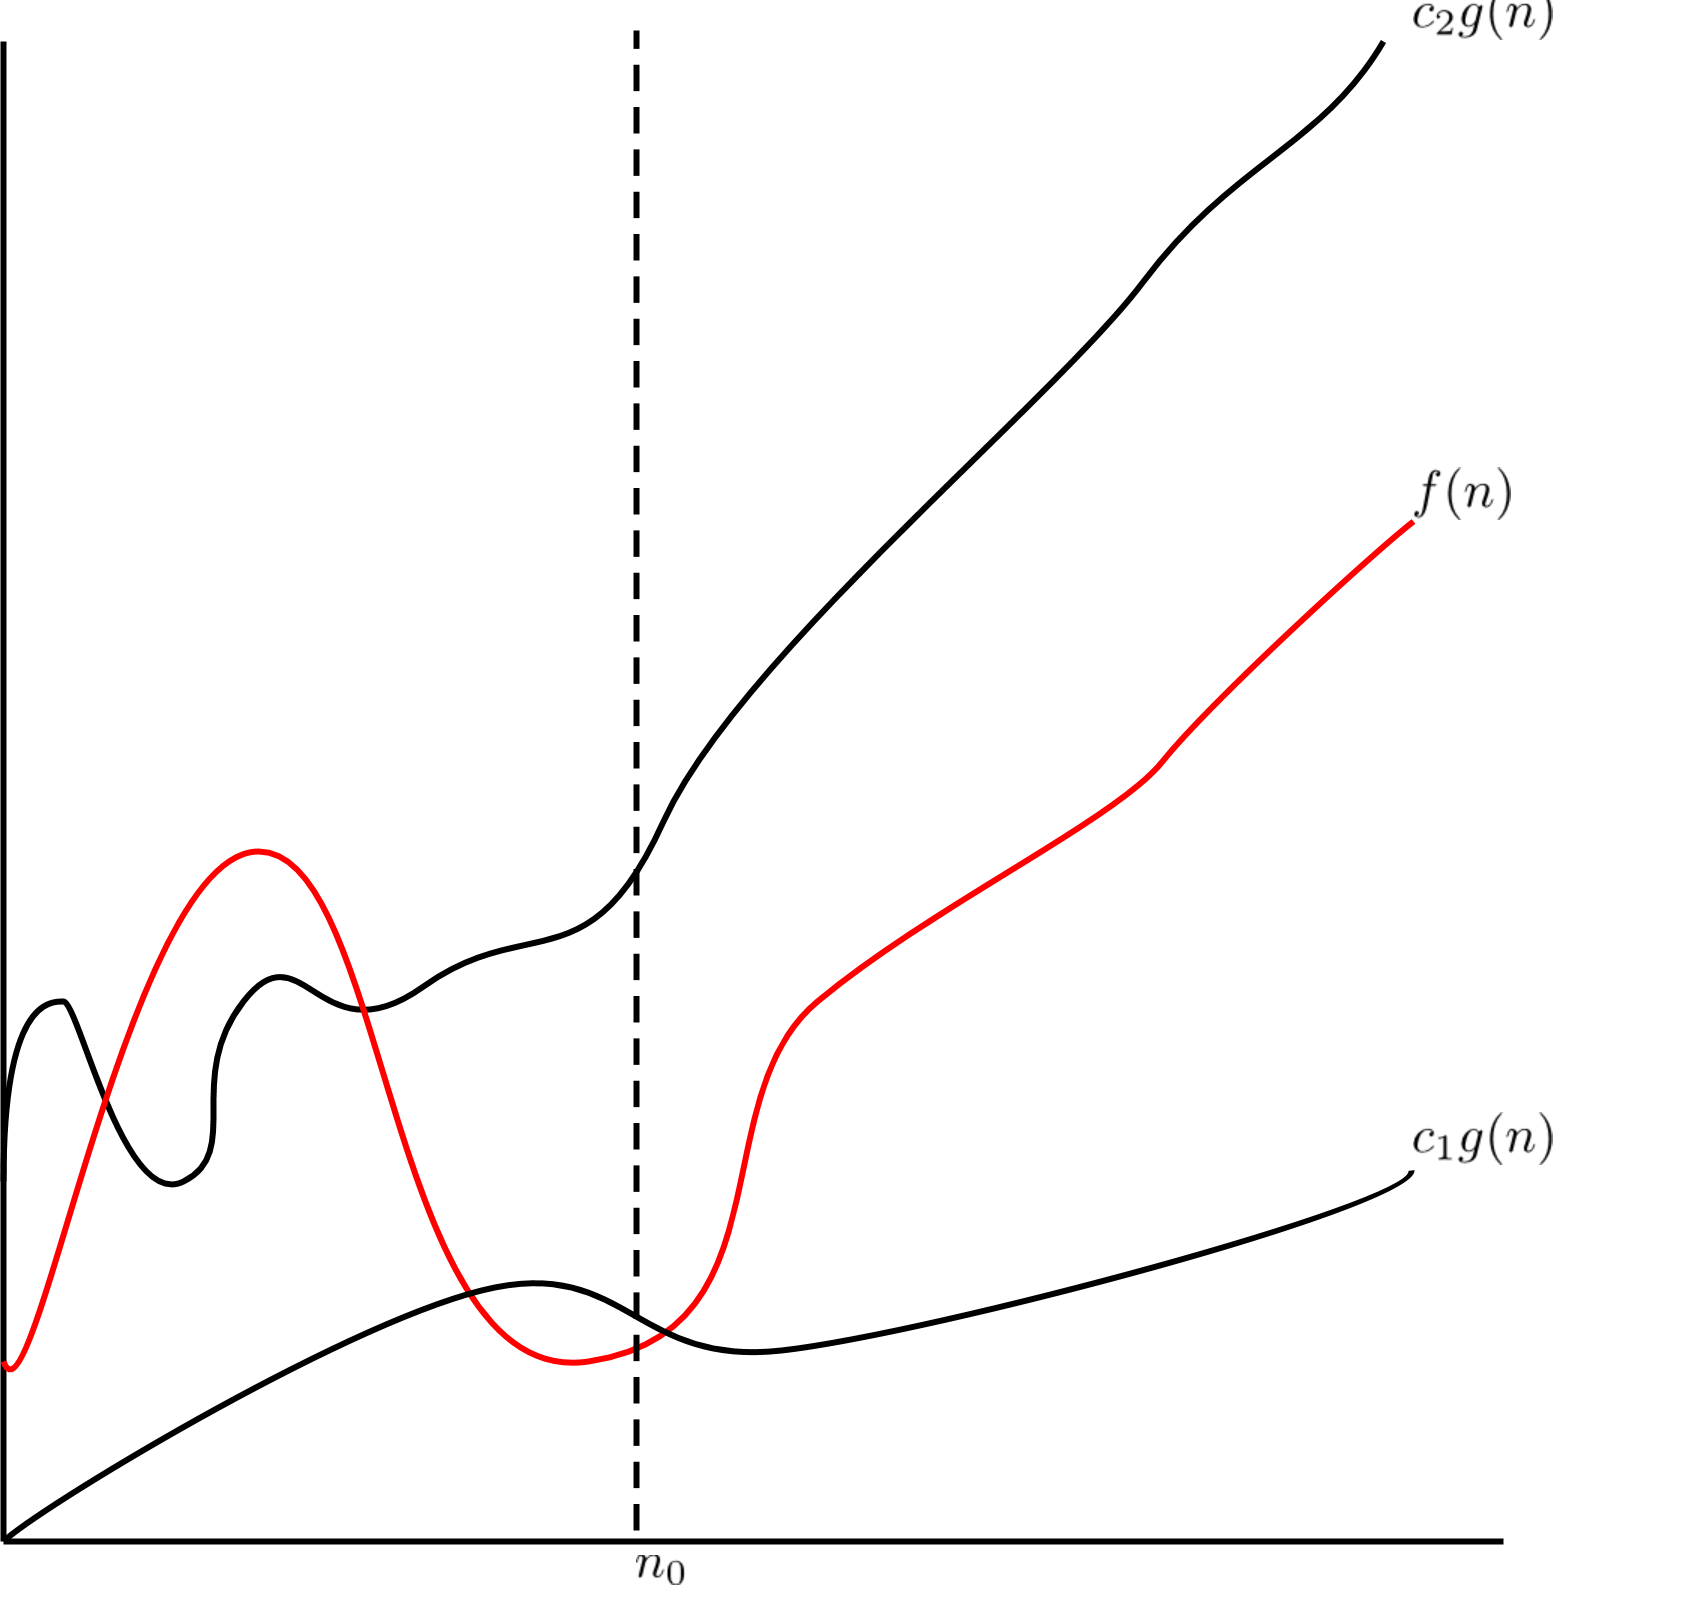
\includegraphics[width=0.80\textwidth]{img/plots/plottheta.png}
\end{center}

\paragraph{Esempi}
\begin{align*}
	f_1(n) = & 2n^2 + 5n + 3 = \Theta (n^2) && f_1(n) \neq \Theta (n^3) \\
	& c_1 = 1 \quad c_2 = 3 \quad n_0 = 6 && f_1(n) = O(n^3) \\
	f_2(n) = & 2 + \sin (n) = \Theta (1) && f_1(n) \neq \Omega (n^3) \\
	& c_1 = 1 \quad c_2 = 3 \quad n_0 = 0 && \qquad \Downarrow \\
	& && \frac{f_1(n)}{n_3} \rightarrow 0
\end{align*}
\newpage
\subsection{Metodo del limite}
$f(n),g(n) > 0 \quad \forall n$ \par \medskip
Se $\lim_{n \to +\infty} \frac{f(n)}{g(n)}$ esiste, allora:

\begin{enumerate}
	\item Se $\lim_{n \to +\infty} \frac{f(n)}{g(n)} = k > 0$ allora $f(n) = \Theta \big( g(n) \big)$.\par
	\begin{align*}
		\text{Infatti } \forall \varepsilon > 0 \ \exists n_0 : \forall n \geq n_0 & \Rightarrow \abs{\frac{f(n)}{g(n)} - k} \leq \varepsilon \\
		& \Rightarrow - \varepsilon \leq \frac{f(n)}{g(n)} - k \leq \varepsilon 
	\end{align*}
	\begin{gather*}
		k - \varepsilon \leq \frac{f(n)}{g(n)} \leq k + \varepsilon \\
		(k - \varepsilon)g(n) \leq f(n) \leq (k + \varepsilon)g(n) \qquad \text{per } 0 < \varepsilon < k
	\end{gather*}
	
	\item Se $\lim_{n \to +\infty} \frac{f(n)}{g(n)} = 0$ allora $f(n) = O \big( g(n) \big)$ e 
	$f(n) \neq \Omega \big( g(n) \big)$.
	
	\item Se $\lim_{n \to +\infty} \frac{f(n)}{g(n)} = \infty$ allora $f(n) = \Omega \big( g(n) \big)$ e 
	$f(n) \neq O \big( g(n) \big)$.
\end{enumerate}

\subsection{Alcune proprietà generali}
\begin{itemize}
	\item $f(n) = a_kn^k + a_{k-1}n^{k-1} + \dots + a_1n + a_0 = \Theta (n^k)$
	\item $h \neq k \quad \Theta (n^h) \neq \Theta (n^k)$
	\item $a \neq b \quad \Theta (a^k) \neq \Theta (b^n)$
	\item $h \neq k \quad \Theta (a^{n+h}) = \Theta (a^{n+k})$
	\item $a \neq b \quad \Theta (\log_an) = \Theta (\log_bn)$
\end{itemize} 
In generale
\begin{gather*}
	O(1) \subseteq O(\log n) \subseteq O(n) \subseteq O(n \log n) \subseteq O(n^2) \subseteq \dots
\end{gather*}
Rivediamo \texttt{Insertion Sort} con le notazioni asintotiche:
\begin{displaymath}
	T^{IS}(n) = O(n^2) \qquad T^{IS}_{max}(n) = \Theta (n^2)
\end{displaymath}
Vale anche la proprietà seguente:
\begin{align*}
	2n^k + \Theta (n^{k-1}) = O(n^k) (&\subseteq \Theta (n^k)) \\
	& = \Theta (n^k) \quad \forall k > 0
\end{align*}
\section{Lezione del 09/03/2018}

\subsection{Complessità di un problema}
Dato un problema\footnote{Relazione/funzione INPUT $\rightarrow$ OUTPUT} P ci sono
(possono esserci) algoritmi che risolvono P. La \textbf{complessità} di P è la 
complessità dell'algoritmo di complessità più bassa che lo risolve.

\paragraph{Limite superiore per complessità di P} Se A è un algoritmo per P con
complessità $f(n)$, allora P è $O \big( f(n) \big)$. \par \smallskip
Vediamo un paio di esempi:
\begin{itemize}
	\item \texttt{Insertion Sort} algoritmo di ordinamento $O(n^2)$;
	\item \texttt{Merge Sort} algoritmo di ordinamento $O(n \log n)$;
\end{itemize}

\paragraph{Limite inferiore per complessità di P}
Se \underline{ogni} algoritmo che risolve P ha complessità $\Omega \big( f(n) \big)$ allora 
P è $\Omega \big( f(n) \big)$
\bigskip

$\implies$ se P è $O \big( f(n) \big)$ e $\Omega \big( f(n) \big) \Rightarrow$ P è $\Theta \big( f(n) \big)$ 

\subsection{Esempio: limite inferiore per l'ordinamento basato su scambi}

\paragraph{Def (inversione)} Dato \texttt{A[1$\twodots$n]}, una \emph{inversione} è una coppia $(i,j)$
con $i,j \in [1,n]$ con $i < j$ e \texttt{A[i]} $>$ \texttt{A[j]}.\par \medskip
Operazione disponibile: \texttt{A[k]} $\leftrightarrow$ \texttt{A[k+1]} (scambio tra gli elementi in posizione
$k$ e $k+1$).
\begin{align*}
	\# inv(A) & = \text{numero di inversioni di } A \\
	& = \abs{\{ (i,j) \ \vert \ 1 \leq i \leq j \leq n \land A[i] > A[j] \}}
\end{align*}

\begin{enumerate}
	\item A è ordinato sse $\# inv(A) = 0$;
	\item A è ordinato in senso inverso sse 
	\begin{displaymath}
		\displaystyle\sum_{j=2}^{n}j-1 = \displaystyle\sum_{j=1}^{n-1}j = \frac{n(n-1)}{2}
	\end{displaymath}
	Ossia, $\# inv(A)$ è massimizzato.
\end{enumerate}

Vediamo cosa succede alle coppie $(i,j)$ e a $\# inv(A)$ nel caso avvenga uno scambo \texttt{A[k]}
$\leftrightarrow$ \texttt{A[k+1]}.

\begin{itemize}
	\item $i,j \neq k$ e $i,j \neq k+1 \implies (i,j)$ è inversione prima sse è inversione dopo;
	\item $i = k, \ j = k+1$
	\[ \implies
	\begin{cases}
		A[k] < A[k+1] & \quad +1 \text{ inversione} \\
		A[k] = A[k+1] & \quad \# inv(A) \text{ non cambia} \\
		A[k] > A[k+1] & \quad -1 \text{ inversione}
	\end{cases}
	\]
	\item $i = k$ oppure $i = k+1$, $j > k+1 \implies (k,j)$ è inversione prima sse $(k+1,j)$ è
	inversione dopo;
	\item $j = k$ oppure $j = k+1$, $i < k$, analogo al caso precedente.
\end{itemize}

Per concludere, possiamo dire che l'operazione \texttt{A[k]} $\leftrightarrow$ \texttt{A[k+1]}
riduce $\# inv(A)$ al massimo di 1.
\begin{displaymath}
	\implies \text{qualunque algoritmo di ordinamento è } \Omega \Big(\frac{n(n-1)}{2} \Big) = \Omega (n^2)
\end{displaymath}
\texttt{Insertion Sort} è ``quasi'' basato su scambi $\Rightarrow \text{è } O(n^2) \Rightarrow \text{è } \Theta (n^2)$

\subsection{Soluzione di ricorrenze}
Abbiamo visto per \texttt{Merge Sort} la complessità nel modo seguente:

\begin{codebox}
	\Procname{$\proc{Merge-Sort}(A,p,r)$}
	\li \If $p < r$
	\li     \Then
	$q \gets \floor{\frac{(p + r)}{2}}$ 
	\li         $\proc{Merge-Sort}(A,p,q)$
	\li         $\proc{Merge-Sort}(A,q+1,r)$
	\li         $\proc{Merge}(A,p,q,r)$
	\Comment complessità $an + b$
	\End
\end{codebox}

\[ T^{MS}(n) =
\begin{cases}
c_0       & \quad \text{se } n \leq 1 \\
T^{MS}(\floor{\frac{n}{2}})+T^{MS}(\ceil{\frac{n}{2}}) + an + b  & \quad \text{se } n>1
\end{cases}
\]

È stato tuttavia un approccio non molto preciso. Ci sono due metodi per risolvere precisamente 
i problemi di ricorrenza:
\begin{itemize}[noitemsep]
	\item \emph{Metodo di sostituzione} (\ref{ricorrenze:sostituzione});
	\item \emph{Master Theorem}.
\end{itemize}

\subsubsection{Metodo di sostituzione} \label{ricorrenze:sostituzione}
Dato una ricorrenza, si può provare a ``indovinare'' la soluzione, oppure si può sviluppare l'\emph{albero %
delle ricorrenze}:
\begin{itemize}
	\item \emph{radice}: chiamata di cui vogliamo la complessità;
	\item per ogni nodo:
	\begin{itemize}
		\item[$\rightarrow$] costo della parte non ricorsiva;
		\item[$\rightarrow$] un figlio per ogni chiamata.
	\end{itemize}
\end{itemize}

\paragraph{Esempio} 

\[ T(n) =
\begin{cases}
4       & \quad \text{se } n = 1 \\
2T(\frac{n}{2})+ 6n  & \quad \text{se } n>1
\end{cases}
\]

Proviamo ad ``indovinare'' la soluzione\footnote{In classe, è stato visto anche un esempio con un albero. Ho scelto di ometterlo per la poca praticità nel rappresentarlo in \LaTeX.}. Assomiglia a \texttt{Merge Sort},
quindi ipotizziamo abbia una complessità con un andamento simile a 
\begin{displaymath}
	T(n) = an \log n + bn + c
\end{displaymath}
Facciamo la prova induttiva.

\begin{align*}
	(n = 1) \quad T(1) & = 4 \\
	& = a \cdot 1 \cdot \log 1 + b \cdot + c \\
	& = b + c && \text{ok se } b + c = 4 \\
	(n > 1) \quad T(n) & = 2T \big( \frac{n}{2} \big) + 6n \\
\end{align*}
\begin{align*}
	\text{Per ipotesi induttiva} \\
	T \big( \frac{n}{2} \big) & = a \frac{n}{2} \cdot \log \frac{n}{2} + b \frac{n}{2} + c \\
	\text{Calcolo ora } T(n) \\
	T(n) & = an \log_2 \frac{n}{2} + bn + 2c + 6n = \\
	& = an \log_2n - an \log_22 + bn + 6n + 2c = \\
	& = an \log_2n + n(b + 6 - a) + 2c \\
	& = an \log_2n + bn + c \\
	& \qquad \Downarrow
\end{align*}
\begin{align*}
	b + 6 - a = b \Rightarrow & a = 6 \\
	2c = c \Rightarrow & c = 0 \\
	& b + c = 4 \Rightarrow b = 4 \\
	T(n) &= an \log n + bn + c \\
	&= 6n \log n + 4n
\end{align*}

%glossaries
%\glsaddall
%\printglossaries

\end{document}